\section{Исследовательский раздел}
\setcounter{figure}{0}
\setcounter{table}{0}
\subsection{Сравнение результатов работы метода с существующим аналогом}

Сравнение результатов работы метода по определению темпа музыки производилось с результатами работы метода beat\_track() из библиотеки librosa. Этот метод определяет средний темп для указанного аудиофайла, поэтому для сравнения аудиозапись также разделялась на 5-секундные фрагменты, для каждой из которых вызывался этот метод.

Исследование проводилось на 8 аудиофайлах с переменным темпом и на 8 с постоянным. Все аудиофайлы были сгруппированы по жанрам. Таким образом, в случае с переменным темпом использовались музыкальные композиции в поп, рок и соул жанрах, а в случае с постоянным темпом -- в фанк, джаз, поп и рок жанрах.

На рисунках~\ref{img:tempo_librosa_change} -- \ref{img:tempo_librosa_const} представлены гистограммы, отображающие точность оценки переменного и постоянного темпа исследуемых программных решений.

Как видно из гистограмм, разработанный метод превосходит библиотеку в точности оценки переменного темпа музыки, но при этом в точности определения постоянного темпа в большинстве случаев уступает аналогу.

\begin{figure}[h]
	\centering
	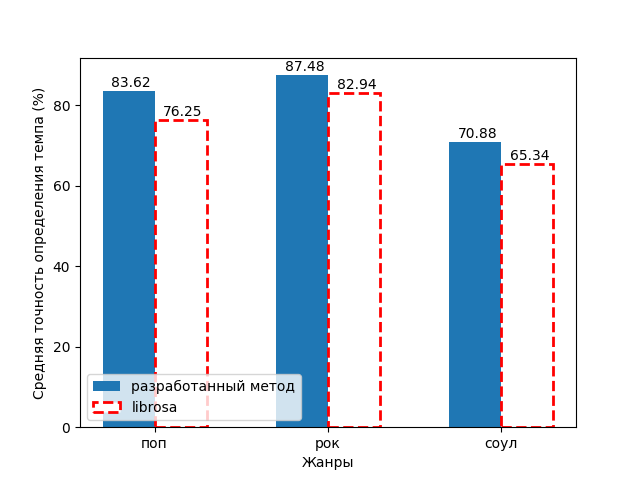
\includegraphics[scale=0.9]{../graphs/changing_tempo_librosa.png}
	\caption{Точность результатов работы ПО и аналога при переменном темпе}
	\label{img:tempo_librosa_change}
\end{figure}

\begin{figure}[h]
	\centering
	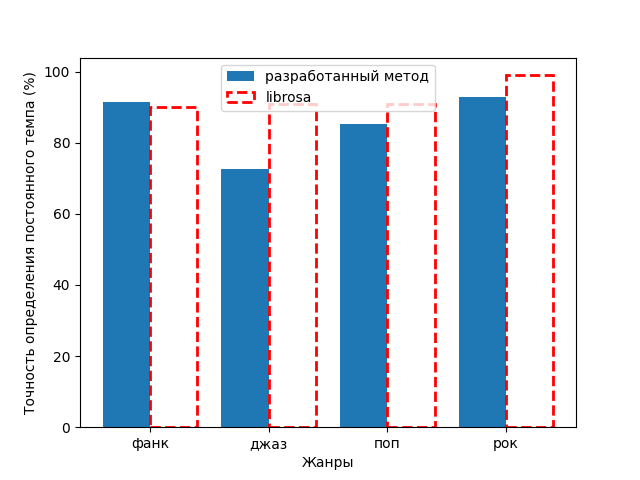
\includegraphics[scale=0.9]{../graphs/const_tempo_librosa.png}
	\caption{Точность результатов работы ПО и аналога при постоянном темпе}
	\label{img:tempo_librosa_const}
\end{figure}
\clearpage
\subsection{Применимость ПО для аудиозаписей с разным набором инструментов}

В качестве тестовых данных для анализа ритма использовались аудиофайлы со следующими инструментами:
 
\begin{enumerate}
	\item Только ударные.
	\item Только гитара.
	\item Гитара вместе с ударными.
\end{enumerate}

Во всех трех аудиозаписях использовался один и тот же музыкальный фрагмент с переменным размером (3/4 первые 15 секунд и 4/4 оставшееся время) (см. рис.~\ref{img:hz_ref}).

\begin{figure}[h]
	\centering
	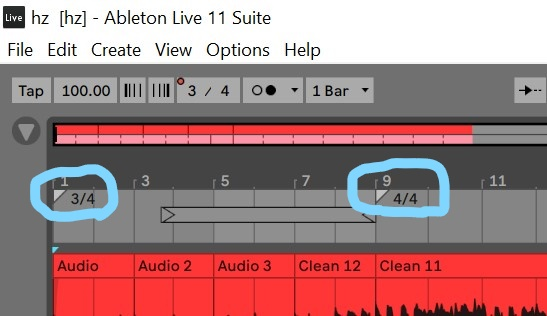
\includegraphics[scale=0.7]{inc/img/hz_ref.jpg}
	\caption{Эталонные значения размера}
	\label{img:hz_ref}
\end{figure}

%\newpage

Результаты работы ПО по определению переменного размера для трех указанных аудиофайлов представлены в таблицах~\ref{tab:hz_drums} -- \ref{tab:hz_full} соответственно.

\begin{table}[!h]
	\begin{center}
		\caption{\label{tab:hz_drums}Результаты для 1-го аудиофайла}
		\begin{tabular}{|p{8cm}|p{8cm}|}
			\hline
			Время (с) & Размер\\
			\hline
			0 & 3/4\\
			\hline
			15 & 4/4\\
			\hline
		\end{tabular}
	\end{center}
\end{table}

\begin{table}[!h]
	\begin{center}
		\caption{\label{tab:hz_guitar}Результаты для 2-го аудиофайла}
		\begin{tabular}{|p{8cm}|p{8cm}|}
			\hline
			Время (с) & Размер\\
			\hline
			0 & 2/4\\
			\hline
			5 & 3/4\\
			\hline
			10 & 2/4\\
			\hline
			20 & 1/4\\
			\hline
		\end{tabular}
	\end{center}
\end{table}

\begin{table}[!h]
	\begin{center}
		\caption{\label{tab:hz_full}Результаты для 3-го аудиофайла}
		\begin{tabular}{|p{8cm}|p{8cm}|}
			\hline
			Время (с) & Размер\\
			\hline
			0 & 2/4\\
			\hline
			5 & 3/4\\
			\hline
			15 & 4/4\\
			\hline
			20 & 2/4\\
			\hline
		\end{tabular}
	\end{center}
\end{table}

\newpage

На рисунке~\ref{img:measure_instr} приведена средняя точность оценки тактового размера (в процентах) в зависимости от набора инструментов в аудиозаписи.

\begin{figure}[h]
	\centering
	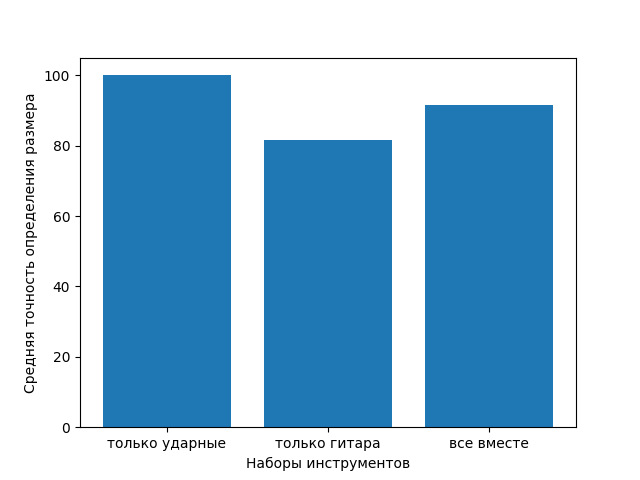
\includegraphics[scale=0.89]{../graphs/measure_instr.png}
	\caption{точность оценки размера в зависимости от инструментов}
	\label{img:measure_instr}
\end{figure}

\newpage

Как видно из гистограммы, наибольшую точность программа выдает на аудиофайле с ударными, а наименьшую -- на аудиозаписи с гитарой. Такие результаты могут быть связаны с небольшими отклонениями гитары от ритмической сетки, а также со смещением сильных долей в гитарной партии. При этом во всех случаях точность определения тактового размера лежит в допустимых пределах ($\ge82\%$).

Для анализа темпа в свою очередь использовались аудиофайлы со следующими инструментами:

\begin{enumerate}
	\item Только ударные.
	\item Гитары и бас.
	\item Ударные, бас и гитара.
	\item Полный фрагмент (ударные, бас, гитара и вокал).
\end{enumerate}

Здесь использовался другой музыкальный фрагмент, также одинаковый для всех трех аудиофайлов, с переменным темпом (115 bpm первые 25 секунд и 120 bpm оставшееся время) (<<Toxicity>> - System of a down).

Результаты работы ПО по определению переменного темпа для этих аудиофайлов представлены в таблицах~\ref{tab:soad_drums} -- \ref{tab:soad_full} соответственно.

\begin{table}[!h]
	\begin{center}
		\caption{\label{tab:soad_drums}Результаты для 1-го аудиофайла}
		\begin{tabular}{|p{8cm}|p{8cm}|}
			\hline
			Время (с) & Темп (bpm)\\
			\hline
			0 & 105\\
			\hline
			30 & 113\\
			\hline
			35 & 105\\
			\hline
			40 & 113\\
			\hline
			45 & 105\\
			\hline
		\end{tabular}
	\end{center}
\end{table}

\begin{table}[!h]
	\begin{center}
		\caption{\label{tab:soad_guitar}Результаты для 2-го аудиофайла}
		\begin{tabular}{|p{8cm}|p{8cm}|}
			\hline
			Время (с) & Темп (bpm)\\
			\hline
			0 & 91\\
			\hline
			30 & 186\\
			\hline
			35 & 91\\
			\hline
			40 & 160\\
			\hline
			45 & 91\\
			\hline
		\end{tabular}
	\end{center}
\end{table}

\begin{table}[!h]
	\begin{center}
		\caption{\label{tab:soad_minus}Результаты для 3-го аудиофайла}
		\begin{tabular}{|p{8cm}|p{8cm}|}
			\hline
			Время (с) & Темп (bpm)\\
			\hline
			0 & 131\\
			\hline
			5 & 103\\
			\hline
			10 & 131\\
			\hline
			15 & 103\\
			\hline
			20 & 131\\
			\hline
		\end{tabular}
	\end{center}
\end{table}

\begin{table}[!h]
	\begin{center}
		\caption{\label{tab:soad_full}Результаты для 4-го аудиофайла}
		\begin{tabular}{|p{8cm}|p{8cm}|}
			\hline
			Время (с) & Темп (bpm)\\
			\hline
			0 & 103\\
			\hline
			5 & 93\\
			\hline
			10 & 103\\
			\hline
			15 & 93\\
			\hline
		\end{tabular}
	\end{center}
\end{table}

\newpage

На рисунке~\ref{img:tempo_instr} приведена средняя точность оценки темпа в зависимости от набора инструментов в аудиозаписях для разработанного ПО.

\begin{figure}[h]
	\centering
	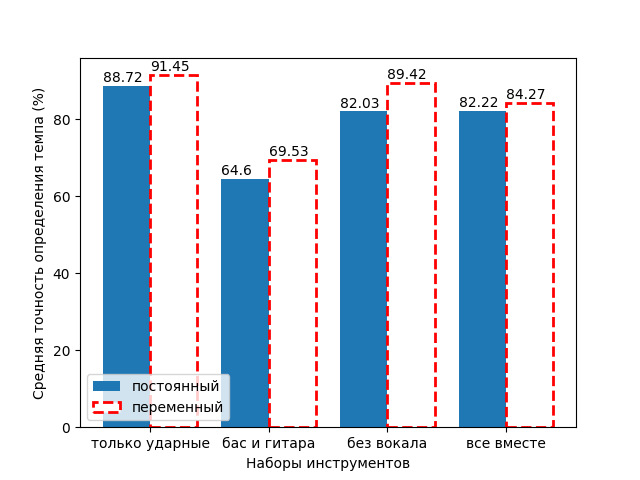
\includegraphics[scale=1]{../graphs/tempo_instr.png}
	\caption{точность оценки темпа в зависимости от инструментов}
	\label{img:tempo_instr}
\end{figure}

%\newpage

Как видно из гистограммы, наилучшие результаты разработанная программа показывает на аудизаписи, содержащей только ударные, и на аудиозаписи без вокала (с ударными, басом и гитарой). Наименьшая точность результатов получилась на аудиофайле, содержащем только гитару и бас. Помимо перечисленных ранее причин, это может быть связано также с проблемами в качестве этой записи.

\newpage

\subsection{Применимость ПО для музыки разных жанров}

Для исследования работы ПО в данном случае использовались следующие жанры:

\begin{itemize}
	\item[---] поп;
	\item[---] рок;
	\item[---] фанк;
	\item[---] джаз.
\end{itemize}

Примеры результатов работы метода по определению темпа для перечисленных жанров представлены в таблицах~\ref{tab:tempo_genres} -- \ref{tab:tempo_jazz}.

\begin{table}[!h]
	\begin{center}
		\caption{\label{tab:tempo_genres}Результаты определения темпа для разных жанров}
		\begin{tabular}{|p{8cm}|p{8cm}|}
			\hline
			\textbf{Жанр} & \textbf{Темп (bpm)}\\
			\hline
			Поп & 118\\
			\hline
			Рок & 113\\
			\hline
			Фанк & 119\\
			\hline
		\end{tabular}
	\end{center}
\end{table}

\begin{table}[!h]
	\begin{center}
		\caption{\label{tab:tempo_jazz}Результаты определения темпа для джаза}
		\begin{tabular}{|p{8cm}|p{8cm}|}
			\hline
			\textbf{Время (с)} & \textbf{Темп (bpm)}\\
			\hline
			0 & 85\\
			\hline
			5 & 99\\
			\hline
			30 & 85\\
			\hline
			35 & 99\\
			\hline
			60 & 128\\
			\hline
			65 & 99\\
			\hline
			80 & 128\\
			\hline
			85 & 191\\
			\hline
			90 & 87\\
			\hline
			95 & 33\\
			\hline
			100 & 99\\
			\hline
			115 & 191\\
			\hline
			120 & 99\\
			\hline
		\end{tabular}
	\end{center}
\end{table}

\newpage

Для расчета точности был собран и размечен датасет по 3-5 аудиофайлов для каждого жанра (как для постоянного темпа или ритма, так и для переменного).

\newpage

На рисунке~\ref{img:tempo_genres} представлена точность определения темпа музыки в зависимости от жанра.

\begin{figure}[h]
	\centering
	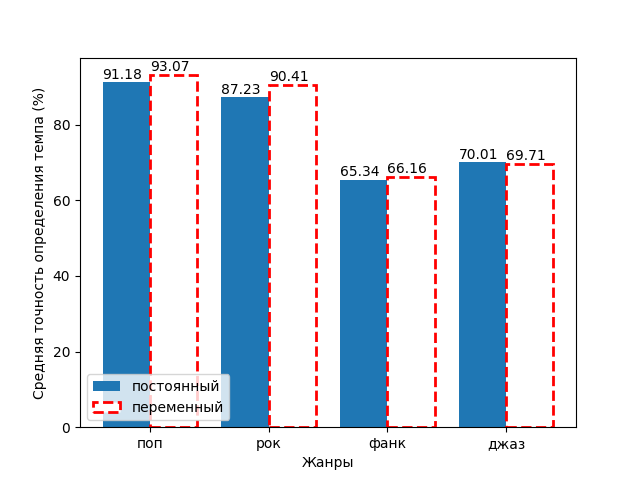
\includegraphics[scale=1]{../graphs/tempo_genres.png}
	\caption{точность оценки темпа в зависимости от жанра}
	\label{img:tempo_genres}
\end{figure}

Пример результатов по определению ритма для тех же жанров приведен в таблице~\ref{tab:rhythm_genres}.

\begin{table}[!h]
	\begin{center}
		\caption{\label{tab:rhythm_genres}Результаты определения ритма для разных жанров}
		\begin{tabular}{|p{8cm}|p{8cm}|}
			\hline
			\textbf{Жанр} & \textbf{Ритм}\\
			\hline
			Поп & 2/4\\
			\hline
			Рок & 2/4\\
			\hline
			Фанк & 5/4\\
			\hline
			Джаз & 3/4\\
			\hline
		\end{tabular}
	\end{center}
\end{table}

\newpage

На рисунке~\ref{img:measure_genres} представлена точность определения тактового размера в зависимости от жанра.

\begin{figure}[h]
	\centering
	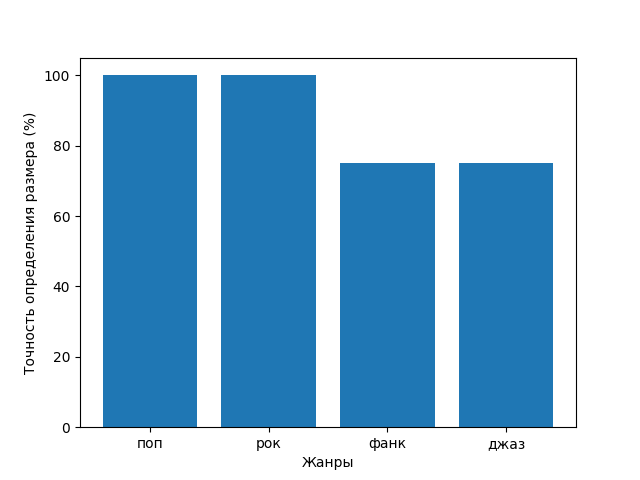
\includegraphics[scale=1]{../graphs/measure_genres.png}
	\caption{точность оценки размера в зависимости от жанра}
	\label{img:measure_genres}
\end{figure}

Как видно из гистограмм, точность оценки темпа и ритма значительно снижается на таких жанрах, как фанк и джаз. Это связано с особенностями этих жанров, такими как смещение ритма и сильных долей, что в свою очередь влияет и на определение темпа.

\subsection{Оценка разработанного метода}

В результате исследований у разработанного метода были выявлены следующие достоинства:

\begin{itemize}
	\item[---] более точное определение переменного темпа в сравнении с библиотечным методом;
	\item[---] высокая точность определения темпа и ритма для аудиозаписей с ударными;
	\item[---] высокая точность определения темпа и ритма для рок и поп музыки.
\end{itemize}

При этом у метода были обнаружены такие недостатки, как:

\begin{itemize}
	\item[---] менее точное определение постоянного темпа по сравнению с библиотечным методом;
	\item[---] более существенные ошибки при оценке темпа и ритма музыки, содержащей только гитары;
	\item[---] большие ошибки при определении тактового размера и темпа музыки таких жанров, как фанк и джаз.
\end{itemize}

\subsection*{Выводы}
В данном разделе был проведён анализ применимости разработанного метода для музыки с разным составом инструментов и разных жанров. 

В результате было выяснено, что наиболее высокой точности определения темпа и ритма метод достигает на музыке, содержащей ударные инструменты, а также в рок и поп жанрах.

Помимо этого, было проведено сравнение результатов разработанного метода с результатами библиотечной функции для определения темпа и выяснено, что разработанный метод превосходит библиотечный в точности при оценке переменного темпа примерно на 15\%.